%%%%%%%%%%%%%%%%%%%%%%%%%%%%%%%%%%%%%%%%%%%%%%%%%%%%%%%%%%%%%%%%%%%%%%%%
% Uni Duesseldorf
% Lehrstuhl fuer Datenbanken und Informationssysteme
% Vorlage fuer Bachelor-/Masterarbeiten
% Optimiert fuer den Original-Latex-Kompiler LATEX.EXE (LaTeX=>PS=>PDF)
%%%%%%%%%%%%%%%%%%%%%%%%%%%%%%%%%%%%%%%%%%%%%%%%%%%%%%%%%%%%%%%%%%%%%%%%
% Ueberarbeitung für pdflatex (LaTeX=>PDF)
%%%%%%%%%%%%%%%%%%%%%%%%%%%%%%%%%%%%%%%%%%%%%%%%%%%%%%%%%%%%%%%%%%%%%%%%
% Vorlage Changelog:
% 10.09.2015 (Matthias Liebeck): Nummerierung des Inhaltsverzeichnis nun römisch, Beispiel für einen Anhang eingebaut, \raggedbottom hinter sections eingefügt
%%%%%%%%%%%%%%%%%%%%%%%%%%%%%%%%%%%%%%%%%%%%%%%%%%%%%%%%%%%%%%%%%%%%%%%%
%%%% BEGINN EINSTELLUNG FUER DIE ARBEIT. UNBEDINGT ERFORDERLICH! %%%%%%%
%%%%%%%%%%%%%%%%%%%%%%%%%%%%%%%%%%%%%%%%%%%%%%%%%%%%%%%%%%%%%%%%%%%%%%%%
% Geben Sie Ihren Namen hier an:
\newcommand{\bearbeiter}{Ole Kiefer}

% Geben Sie hier den Titel Ihrer Arbeit an:
\newcommand{\titel}{Collaborative Filtering}
\newcommand{\titeldeutsch}{Kollaboratives Filtern}



% Geben Sie das Datum des Beginns und Ende der Bachelorarbeit ein:
\newcommand{\beginndatum}{22. Januar 2016}
\newcommand{\abgabedatum}{01.~M\"{a}rz~2016}

% Geben Sie die Namen des Erst- und Zweitgutachters an:
\newcommand{\erstgutachter}{Prof. Dr.~Stefan Harmeling}
\newcommand{\zweitgutachter}{Prof. Dr.~Stefan Conrad}

% Falls Sie die Arbeit zweiseitig ausdrucken wollen,
% benutzen Sie die folgende Zeile mit
% \AN fuer zweiseitigen Druck
% \AUS fuer einseitigen Druck
\newcommand{\zweiseitig}{\AN}

% Falls die Arbeit in englischer Sprache verfasst 
% werden soll, dann benutzen Sie die folgende Zeile mit
% englisch fuer englische Sprache
% deutsch fuer deutsche Sprache
\newcommand{\sprache}{deutsch}

% Hier wird eingestellt, ob es sich bei der Arbeit um eine Bachelor- 
% oder Masterarbeit handelt (unpassendes auskommentieren!):
\newcommand{\arbeit}{Bachelorarbeit}
%~ \newcommand{\arbeit}{Masterarbeit}




%%%%%%%%%%%%%%%%%%%%%%%%%%%%%%%%%%%%%%%%%%%%%%%%%%%%%%%%%%%%%%%%%%%%%%%%
%%%% ENDE EINSTELLUNGEN %%%%%%%%%%%%%%%%%%%%%%%%%%%%%%%%%%%%%%%%%%%%%%%%
%%%%%%%%%%%%%%%%%%%%%%%%%%%%%%%%%%%%%%%%%%%%%%%%%%%%%%%%%%%%%%%%%%%%%%%%

% Die folgende Zeile NICHT EDITIEREN oder loeschen


%%%%%%%%%%%%%%%%%%%%%%%%%%%%%%%%%%%%%%%%%%%%%%%%%%%%%%%%%%%
% Obere Titelmakros. Editieren Sie diese Datei nur, wenn
% Sie sich ABSOLUT sicher sind, was Sie da tun!!!
% (Z.B. zum Abaendern der BA-Vorlage in eine MA-Vorlage)
% Uni Duesseldorf
% Lehrstuhl fuer Datenbanken und Informationssysteme
% Version 2.2 - 2.3.2010
%%%%%%%%%%%%%%%%%%%%%%%%%%%%%%%%%%%%%%%%%%%%%%%%%%%%%%%%%%%
\newcommand{\AN}{twoside}
\newcommand{\AUS}{}
%\newcommand{\englisch}{}
%\newcommand{\deutsch}{\usepackage[german]{babel}}

%% Die folgenden auskommentierten Optionen dienen der automatischen
%% Erkennung des Latex-Kompilers und dem Setzen der davon abhängigen
%% Einstellungen. Bei Problem z.B. mit dem Einbinden von verschiedenen
%% Grafiktypen bei Verwendung von PdfLatex oder Latex, einfach die
%% verschiedenen \usepackage(s) ausprobieren. (Mit diesen Einstellungen
%% funktionierte diese Vorlage bei der Verwenundg von latex.exe als
%% Kompiler bei den meisten Studierenden.)

%\newif\ifpdf \ifx\pdfoutput\undefined
%\pdffalse % we are not running pdflatex
%\else
%\pdfoutput=1 % we are running pdflatex
%\pdfcompresslevel=9 % compression level for text and image;
%\pdftrue \fi

\documentclass[12pt,a4paper, \zweiseitig]{article}

%\usepackage[iso]{umlaute}
\usepackage[utf8x]{inputenc}
\usepackage{palatino} % palatino Schriftart
%\usepackage{makeidx} % um ein Index zu erstellen
\usepackage[nottoc]{tocbibind}
\usepackage[T1]{fontenc} %fuer richtige Trennung bei Umlauten
\usepackage{fancybox} % fuer die Rahmen
\usepackage{shortvrb}
\usepackage{ifthen}
\ifthenelse{\equal{\sprache}{deutsch}}{\usepackage[ngerman]{babel}}{}

\usepackage{a4wide} % ganze A4 Weite verwenden


%%%%%%%  Eigene Pakete %%%%%%%%
%%%%%%%%%%%%%%%%%%%%%%%%%%%%%%%%%%%%%%
%%%%%%  eigene Packages  %%%%%%%%%%%%%
%%%%%%%%%%%%%%%%%%%%%%%%%%%%%%%%%%%%%%

\usepackage[ngerman,pdfauthor={Ole Kiefer},  pdfauthor={Ole Kiefer}, pdftitle={Collaborative Filtering}, pdfkeywords={Bachelor Arbeit, Collaborative Filtering, Kollaboratives Filtern, HHU} breaklinks=true,baseurl={http://www.bretschneidernet.de/tips/thesislatex.html}]{hyperref}





\usepackage{amsmath,amssymb,marvosym} % Mathesachen
\usepackage{listings} % Code Syntax
\usepackage{multirow} % Multirow für Tabellen
\usepackage{algorithm2e} % Algorithmen im Text


% Bilder
\usepackage{placeins} % Grafik Platzierung
\usepackage{graphicx} % Bilder
\usepackage{color} % Farben
\graphicspath{{bilder/}}
\DeclareGraphicsExtensions{.pdf,.png,.jpg} % bevorzuge pdf-Dateien
\usepackage{subcaption}  % mehrere Abbildungen nebeneinander/übereinander

\usepackage[all]{hypcap} % Beim Klicken auf Links zum Bild und nicht zu Caption gehen


\newcommand{\todo}[1]{
	{\colorbox{red}{ TODO: #1 }}
}
\newcommand{\todotext}[1]{
	{\color{red} TODO: #1} \normalfont
}

%\ifpdf
%\usepackage[pdftex,xdvi]{graphicx}
%\usepackage{thumbpdf} %thumbs fuer Pdf
%\usepackage[pdfstartview=FitV]{hyperref} %anklickbares Inhaltsverzeichnis
%\else
%\usepackage[dvips,xdvi]{graphicx}
\usepackage{graphicx}
\usepackage{hyperref} %anklickbares Inhaltsverzeichnis
%\fi

%%%%%%%%%%%%%%%%%%%%%%% Massangaben fuer die Arbeit %%%%%%%%%%%%%%%
\setlength{\textwidth}{15cm}

\setlength{\oddsidemargin}{35mm}
\setlength{\evensidemargin}{25mm}

\addtolength{\oddsidemargin}{-1in}
\addtolength{\evensidemargin}{-1in}

%\makeindex

\begin{document}

%\setcounter{secnumdepth}{4} %Nummerieren bis in die 4. Ebene
%\setcounter{tocdepth}{4} %Inhaltsverzeichnis bis zur 4. Ebene

\pagestyle{headings}

\sloppy % LaTeX ist dann nicht so streng mit der Silbentrennung
%~ \MakeShortVerb{\§}

\parindent0mm
\parskip0.5em


{
\textwidth170mm 
\oddsidemargin30mm 
\evensidemargin30mm 
\addtolength{\oddsidemargin}{-1in}
\addtolength{\evensidemargin}{-1in}

\parskip0pt plus2pt

% Die Raender muessen eventuell fuer jeden Drucker individuell eingestellt
% werden. Dazu sind die Werte fuer die Abstaende `\oben' und `\links' zu
% aendern, die von mir auf jeweils 0mm eingestellt wurden.

%\newlength{\links} \setlength{\links}{10mm}  % hier abzuaendern
%\addtolength{\oddsidemargin}{\links}
%\addtolength{\evensidemargin}{\links}

\begin{titlepage}
\vspace*{-1.5cm}
  \raisebox{17mm}{
    \begin{minipage}[t]{70mm}
      \begin{center}
        %\selectlanguage{german}
        {\Large INSTITUT FÜR INFORMATIK\\}
        {\normalsize
          Computer Vision, Computer Graphics and Pattern Recognition\\
        }
        \vspace{3mm}
        {\small Universitätsstr. 1\\ D--40225 Düsseldorf\\}
     \end{center}
    \end{minipage}
  }
  \hfill
  
\includegraphics[width=130pt]{bilder/HHU_Logo}
  \vspace{14em}

% Titel
  \begin{center}
      	\baselineskip=55pt
    	\textbf{\huge \titel}\\
    	\textbf{\huge \titeldeutsch}
  	 	\baselineskip=0 pt
   \end{center}

  %\vspace{7em}

\vfill

% Autor
  \begin{center}
    \textbf{\Large
      \bearbeiter
    }
  \end{center}

  \vspace{35mm}
 
% Prüfungsordnungs-Angaben
  \begin{center}
    %\selectlanguage{german}
    
%%%%%%%%%%%%%%%%%%%%%%%%%%%%%%%%%%%%%%%%%%%%%%%%%%%%%%%%%%%%%%%%%%%%%%%%%
% Ja, richtig, hier kann die BA-Vorlage zur MA-Vorlage gemacht werden...
% (nicht mehr nötig!)
%%%%%%%%%%%%%%%%%%%%%%%%%%%%%%%%%%%%%%%%%%%%%%%%%%%%%%%%%%%%%%%%%%%%%%%%%
    {\Large \arbeit}

    \vspace{2em}

    \begin{tabular}[t]{ll}
      Beginn der Arbeit:& \beginndatum \\
      Abgabe der Arbeit:& \abgabedatum \\
      Gutachter:         & \erstgutachter \\
                         & \zweitgutachter \\
    \end{tabular}
  \end{center}

\end{titlepage}

}

%%%%%%%%%%%%%%%%%%%%%%%%%%%%%%%%%%%%%%%%%%%%%%%%%%%%%%%%%%%%%%%%%%%%%
\clearpage
\begin{titlepage}
  ~                % eine leere Seite hinter dem Deckblatt
\end{titlepage}
%%%%%%%%%%%%%%%%%%%%%%%%%%%%%%%%%%%%%%%%%%%%%%%%%%%%%%%%%%%%%%%%%%%%%
\clearpage
\begin{titlepage}
\vspace*{\fill}

\section*{Erklärung}

%%%%%%%%%%%%%%%%%%%%%%%%%%%%%%%%%%%%%%%%%%%%%%%%%%%%%%%%%%%
% Und hier ebenfalls ggf. BA durch MA ersetzen...
% (Auch nicht mehr nötig!)
%%%%%%%%%%%%%%%%%%%%%%%%%%%%%%%%%%%%%%%%%%%%%%%%%%%%%%%%%%%

Hiermit versichere ich, dass ich diese \arbeit~
selbstständig verfasst habe. Ich habe dazu keine anderen als die
angegebenen Quellen und Hilfsmittel verwendet.

\vspace{25 mm}

\begin{tabular}{lc}
Düsseldorf, den \abgabedatum \hspace*{2cm} & \underline{\hspace{6cm}}\\
& \bearbeiter
\end{tabular}

\vspace*{\fill}
\end{titlepage}

%%%%%%%%%%%%%%%%%%%%%%%%%%%%%%%%%%%%%%%%%%%%%%%%%%%%%%%%%%%%%%%%%%%%%
% Leerseite bei zweiseitigem Druck
%%%%%%%%%%%%%%%%%%%%%%%%%%%%%%%%%%%%%%%%%%%%%%%%%%%%%%%%%%%%%%%%%%%%%

\ifthenelse{\equal{\zweiseitig}{twoside}}{\clearpage\begin{titlepage}
~\end{titlepage}}{}

%%%%%%%%%%%%%%%%%%%%%%%%%%%%%%%%%%%%%%%%%%%%%%%%%%%%%%%%%%%%%%%%%%%%%
\clearpage
\begin{titlepage}

%%% Die folgende Zeile nicht ändern!
\section*{\ifthenelse{\equal{\sprache}{deutsch}}{Zusammenfassung}{Abstract}}
%%% Zusammenfassung:
Beim kollaborativen Filtern versucht man die meist wenigen Informationen einer dünn besetzten Matrix zu verwenden, um diese sinnvoll aufzufüllen. In der Anwendung wird dieses Verfahren beispielsweise benutzt um Vorschläge für einen Nutzer zu kreieren oder Vorlieben eines Nutzers heraus zu finden. Dazu werden Distanzen zwischen den Zeilen oder Spalten der Matrix berechnet um ähnliche Einträge zu finden und neue Informationen zu gewinnen.\\
In dieser Arbeit stelle ich einige gängige Verfahren des kollaborativen Filterns vor, wie den Pearson Correlation Coefficient, Adjusted Cosine Similarity oder den Slope One Algorithmus. Mit dem Floyd-Warshall-Algorithmus wird eine Idee aus der Graphen-Analyse mit diesem Thema in Verbindung gebracht. Zusätzlich habe ich mir zwei Gedanken gemacht, wie ich die simple Metrik des euklidischen Abstandes verbessern kann, um bessere Ergebnisse mit diesem Algorithmus zu erzielen.\\
Der Vergleichstest arbeitet auf der frei verfügbaren MovieLens-Datenbank 100k, in der 943 User 1682 Filme bewertet haben. Die Datenbank wurde aufgeteilt in eine Trainings- und eine Testmenge. Die Algorithmen berechnen mögliche Filmbewertungen und werden mit der Testmenge verglichen. Der durchschnittliche Fehler dient als Vergleichsgröße wie gut der Algorithmus funktioniert. Zusätzlich vergleiche ich die Verfahren auf einer großen Matrix mit niedrigem Rang, in der viele Zeilen eine Linearkombination einer kleinen Menge linear unabhängiger User sind.\\
Im Kapitel 4 wird erst die Parameterwahl einiger Algorithmen getestet. Die produzierten Fehler werden miteinander verglichen und die Ergebnisse interpretiert, zum Beispiel in welchem Szenario sich welcher Algorithmus eignet. Überraschenderweise kann die Methode mit dem euklidischen Abstand mit Strafe ebenfalls sehr gute Ergebnisse erzielen und schlägt alle Algorithmen außer Slope One, welcher in diesem Szenario die besten Ergebnisse erzielt.\\
Im Anhang ist mein Quellcode zur Auswertung der Datenbank mittels der untersuchten Algorithmen in Python zu finden. In der Recommender Klasse sind alle Algorithmen implementiert. Die Testklasse dient als eine Art Toolbox um den Fehler zur Testmenge zu berechnen.



%%%%%%%%%%%%%%%%%%%%%%%%%%%%%%%%%%%%%%%%%%%%%%%%
% Untere Titelmakros. Editieren Sie diese Datei nur, wenn Sie sich
% ABSOLUT sicher sind, was Sie da tun!!!
%%%%%%%%%%%%%%%%%%%%%%%%%%%%%%%%%%%%%%%%%%%%%%%
\vspace*{\fill}
\end{titlepage}

%%%%%%%%%%%%%%%%%%%%%%%%%%%%%%%%%%%%%%%%%%%%%%%%%%%%%%%%%%%%%%%%%%%%%
% Leerseite bei zweiseitigem Druck
%%%%%%%%%%%%%%%%%%%%%%%%%%%%%%%%%%%%%%%%%%%%%%%%%%%%%%%%%%%%%%%%%%%%%
\ifthenelse{\equal{\zweiseitig}{twoside}}
  {\clearpage\begin{titlepage}~\end{titlepage}}{}
%%%%%%%%%%%%%%%%%%%%%%%%%%%%%%%%%%%%%%%%%%%%%%%%%%%%%%%%%%%%%%%%%%%%%
\clearpage \setcounter{page}{1}
\pagenumbering{arabic}
\setcounter{tocdepth}{3}
\tableofcontents

%\enlargethispage{\baselineskip}
\clearpage
%%%%%%%%%%%%%%%%%%%%%%%%%%%%%%%%%%%%%%%%%%%%%%%%%%%%%%%%%%%%%%%%%%%%%
% Leere Seite, falls Inhaltsverzeichnis mit ungerader Seitenzahl und 
% doppelseitiger Druck
%%%%%%%%%%%%%%%%%%%%%%%%%%%%%%%%%%%%%%%%%%%%%%%%%%%%%%%%%%%%%%%%%%%%%
\ifthenelse{ \( \equal{\zweiseitig}{twoside} \and \not \isodd{\value{page}} \)}
	{\pagebreak \thispagestyle{empty} \cleardoublepage}{\clearpage}



\pagenumbering{arabic}
\setcounter{page}{1}



%%%%%%%%%%%%%%%%%%%%%%%%%%%%%%%%%%%%%%%%%%%%%%%%%%%%%%%%%%%%%%%%%%%%%%%%
%%%% BEGINN TEXTTEIL %%%%%%%%%%%%%%%%%%%%%%%%%%%%%%%%%%%%%%%%%%%%%%%%%%%
%%%%%%%%%%%%%%%%%%%%%%%%%%%%%%%%%%%%%%%%%%%%%%%%%%%%%%%%%%%%%%%%%%%%%%%%

%%%%%%%%%%%%%%%%%%%%%%%%%%%%%%%%%%%%%%%%%%%%%%%%%%%%%%%%%%%%%%%%%%%%%%%%
% Text entweder direkt hier hinein schreiben oder, im Sinne der
% besseren Uebersichtlich- und Bearbeitbarkeit mittels \input die
% einzelnen Textteile hier einbinden.
%%%%%%%%%%%%%%%%%%%%%%%%%%%%%%%%%%%%%%%%%%%%%%%%%%%%%%%%%%%%%%%%%%%%%%%%


\section{Einleitung}\label{s.Einleitung}\raggedbottom 
Jeder Homepagebetreiber hat das Ziel den Benutzer möglichst lange auf der eigenen Homepage zu halten, um möglichst viele Klicks und Werbeeinspielungen zu generieren. Ein Weg dies zu erreichen: personalisierte Webseiten, Werbung und Kaufvorschläge. Eine Online-Zeitung schlägt deshalb beim Lesen eines Artikels weitere Artikel vor, die einen interessieren könnten. Marketing-Firmen analysieren den Benutzer, um mit gezielter Werbung mehr Umsatz zu erzielen. Ein 20-jähriger Mann wird eher Autowerbung interessant finden als Make-Up-Werbung. Online-Shops geben Kaufvorschläge zu Artikeln, die man gerade ansieht oder in den Warenkorb gelegt hat, um weitere Käufe anzuregen. Online-Video- oder Musik-Plattformen schlagen ähnliche Filme oder Musikstücke vor, um den Nutzer zu halten.\\
Die Daten, die nötig sind, um den User zu analysieren und zu bewerten, liefert dieser meistens selbst. Tracker verfolgen jeden Klick, jede Mausbewegung wird mit Timern analysiert, Warenkörbe werden ausgewertet, Cookies speichern Daten für die nächste Sitzung. Daraus lassen sich viele Informationen ableiten, man kann abschätzen, wen man zu Besuch hat und womit man Aufmerksamkeit und letztendlich Klicks erreichen kann. In vielen Bereichen liefern die Benutzer ganz bewusst Informationen. Wenn sie etwas bewerten, ihr Profil ausfüllen oder auf den "`like"'-Button drücken. Hierbei treten jedoch zwei Probleme auf. Sehr wenige Nutzer bewerten regelmäßig und extreme Bewertungen (sehr schlecht oder sehr gut) kommen häufiger vor, als die differenzierten Zwischenstufen.\\
Um verschiedene Musikstücke genauer bewerten zu können, setzt der Musik-Streaming-Dienst PANDORA\footnote{\url{www.pandora.com}} deshalb auf ein Expertensystem. Im Music Genome Project\footnote{\url{http://www.pandora.com/about/mgp}} werden 450 charakteristische Merkmale in Liedern von trainierten Musikern bewertet und analysiert. Studierte Musiker geben hier qualitativ hochwertige Bewertungen ab, um die Musikstücke korrekt zu kategorisieren.\\
Beim kollaborativen Filtern nutzt man diese Informationen über die User und Items, um Interessen zu vergleichen, Ähnlichkeiten zu bewerten und Vorschläge zu erstellen.\\ In dieser Arbeit stelle ich sechs Algorithmen vor und teste diese am MovieLens Datensatz 100k (s.\autoref{s.Datenmenge} \nameref{s.Datenmenge}), um sie miteinander vergleichen zu können.

\clearpage


\section{Algorithmen zum kollaborativen Filtern}\label{s.Algorithmen}\raggedbottom
Beim kollaborativen Filtern ist die grundsätzliche Frage: Wie ähnlich sind sich zwei Objekte?
Mathematisch ausgedrückt fragt man nach der Distanz zweier Objekte. Ein Ansatz ist nach der Distanz zweier User zu fragen, der andere die Ähnlichkeit zweier Items zu untersuchen. Um diese Distanz zu berechnen gibt es verschiedene Ansätze.\\
Betrachtet man die Bewertungen als Matrix R mit den User als Zeilen und den Items als Spalten, so wird die Ähnlichkeit zweier User $u$ und $v$ durch die Distanz ihrer Zeilenvektoren bewertet. Die Distanz zweier Items $i$ und $j$ ist der Abstand der Spaltenvektoren. $r_{u,i}$ sei die Bewertung des User $u$ zum Film i. $\hat{r}_{u,i}$ ist die in den Bereich $[-1,1]\subset \mathbb{R}$ normierte Bewertung .  $R^{user}_{u}$ bezeichne die Menge der Filme, die von $u$ bewertet wurden, $R^{item}_{i}$ die Menge der User die Film $i$ bewertet haben.$\bar{r}^{user}_{u}$ ist seine durchschnittliche Bewertung.
\begin{equation}
\begin{aligned}	
R^{user}_{u}&:=\{i | r_{u,i}>0\} \qquad 
R^{item}_{i}:=\{u | r_{u,i}>0\}\\\\
\bar{r}^{user}_{u}&:= \dfrac{\sum\limits_{i \in R^{user}_{u}}r_{u,i}}{|R^{user}_{u}|} \qquad
\bar{r}^{item}_{i}:= \dfrac{\sum\limits_{u \in R^{item}_{i}}r_{u,i}}{|R^{item}_{i}|}\\\\
\mathrm{min}_{R} &= \min\limits_{(u,i)\in R} r_{u,i} \qquad
\mathrm{max}_{R} = \max\limits_{(u,i)\in R} r_{u,i} \\\\
\hat{r}_{u,i}&:= \dfrac{2(r_{u,i}-\mathrm{min}_{R})-(\mathrm{max}_{R}-\mathrm{min}_{R})}{(\mathrm{max}_{R}-\mathrm{min}_{R})}\\
\label{definition}
\end{aligned}
\end{equation}
Im speziellen Fall der MovieLens-Daten ist $\mathrm{min}_{R} = 1$ und $\mathrm{max}_{R} = 5$, die minimale bzw. maximale Bewertung eines Filmes. \\
Ein einfacher Weg einen neuen Vorschlag zu erzeugen ist den ähnlichsten Nutzer zu User $u$ zu finden und ein Item vorzuschlagen, dass $u$ noch nicht bewertet hat. Um ein wenig mehr Informationen zu nutzen und unabhängiger von persönlichen Vorlieben zu werden, benutzt man nicht nur einen, sondern $k$ ähnliche User. Die Menge der $k$ nächsten Nachbarn, nach dem Abstand sortiert, wird beschrieben durch die folgende Formel.
\begin{equation}
\mathrm{kNN}_{d}(u):=\{v_{n} | n\in \mathbb{N} \land 1\leq n\leq k \land v_{n}\in R \land d(u,v_{1})\leq d(u,v_{2})\leq ... \leq d(u,v_{k})\}
\label{knn}
\end{equation}
Um ein Rating für einen Film zu erzeugen kann man nun den Mittelwert der Bewertungen der $k$ nächsten Nachbarn bilden für diesen Film. 
\begin{equation}
r_{d}(u,i) := \dfrac{\sum\limits_{v \in \mathrm{kNN}_{d}(u)} r_{v,i}}{|\mathrm{kNN}_{d}(u)|}  
\label{rating}
\end{equation}
Diese Formel kann man als Grundformel für User-basierte Verfahren ansehen.\\\\
In den nächsten Abschnitten werden die verschiedenen Algorithmen beschrieben. Die euklidische Distanz dient als Einstieg in die Abstandsberechnung. Die Verfahren Pearson Correlation Coefficient \cite[Kap. 2, S.~23]{G2DM}, Adjusted Cosine Similarity \cite[Kap. 3, S.~16]{G2DM} und Slope One \cite[Kap. 3, S.~28]{G2DM} sind beschrieben in dem Buch "`A Programmer's Guide to Data Mining: The Ancient Art of the Numerati"' \cite{G2DM} von Ron Zacharski, Die Algorithmen Floyd-Warshall und Local-User-Similarity-Global-User-Similarity kommen aus dem Paper "`A collaborative filtering framework based on both local user similarity and global user similarity"' \cite{cf} von Luo, Niu, Shen und Ullrich.\\
Für alle Formeln und Algorithmen gilt die Einschränkung für $R^{user}_{u}\cap R^{user}_{v} \neq \emptyset$ bzw. $R^{item}_{i}\cap R^{item}_{j} \neq \emptyset$. Ist die Schnittmenge zwischen zwei User oder Items leer, wird keine Distanz zwischen diesem Paar definiert.

\subsection{User-basierte Algorithmen}
\subsubsection{Euklidische Distanz}\label{s.euclid}
Eine simple Metrik ist die euklidische Distanz:
	\begin{equation}
	\begin{aligned}
	d_{\mathrm{euclid}}(u,v) := \sqrt{\sum\limits_{i \in R^{user}_{u}\cap R^{user}_{v}} (r_{u,i}-r_{v,i})^2  }
	\qquad \mathrm{, f\ddot{u}r }\quad R^{user}_{u}\cap R^{user}_{v} \neq \emptyset
	\label{euclid}
	\end{aligned}
	\end{equation}

Ist die Schnittmenge zwischen User $u$ und User $v$ leer, so wird keine Distanz zwischen ihnen definiert.
Die euklidische Distanz zwischen zwei Benutzern $u$ und $v$ wird berechnet durch alle Items, die sowohl von User $u$ als auch von User $v$ bewertet wurden. Eine geringe Distanz suggeriert eine hohe Ähnlichkeit. Dies führt jedoch zu dem Problem, dass zwei Personen über die sehr wenig gemeinsame Informationen verfügen, ähnlicher bewertet werden können, als zwei Personen über die man sehr viele gemeinsame Informationen hat. Jede Information die man nutzt, vergrößert im Allgemeinen den Abstand zwischen zwei Objekten.\\
Eine Idee wäre eine Strafe einzubauen für Informationen, die man über den User $u$ kennt, aber über User $v$ nicht.
Ich habe mich dazu entschieden die Distanz zur mittleren Bewertung $\dfrac{1}{2}(\mathrm{max}_{R}-\mathrm{min}_{R})+\mathrm{min}_{R})^2$ als Strafe einzubauen. Als Beispiel: User $u$ hat Film $i$ mit 5 bewertet, User $v$ hat keine Bewertung zu diesem Film abgegeben, so wird der Wert 2 als Fehler addiert.
\begin{equation}
\begin{aligned}
\qquad	d&_{\mathrm{euclidpenalized}}(u,v) := \\ &\sqrt{\sum\limits_{i \in R^{user}_{u}\cap R^{user}_{v}} (r_{u,i}-r_{v,i})^2  + \sum\limits_{i \in R^{user}_{u}\backslash R^{user}_{v}} (r_{u,i}-(\dfrac{1}{2}(\mathrm{max}_{R}-\mathrm{min}_{R})+\mathrm{min}_{R})^2) }
	\label{euclidpenalty}
\end{aligned}
\end{equation}

Eine weitere Möglichkeit Nachbarn zu suchen, die viele Informationen teilen, ist durch die Anzahl der Überschneidungen zu dividieren um eine mittlere Distanz zwischen zwei Items zu ermitteln. Damit wird die euklidische Distanz zum mittleren, quadratischen Fehler.
\begin{equation}
d_{\mathrm{euclidnormalized}}(u,v) := \dfrac{\sqrt{\sum\limits_{i \in R^{user}_{u}\cap R^{user}_{v}} (r_{u,i}-r_{v,i})^2  }}{|R^{user}_{u}\cap R^{user}_{v}|}
\label{euclidmean}
\end{equation}

\subsubsection{Pearson Correlation Coefficient}\label{s.pearson}
Der Pearson Algorithmus errechnet eine Ähnlichkeit zwischen allen User mit Hilfe des Pearson Korrelations Koeffizienten. Der Wert zwischen $[-1,1]\subset \mathbb{R}$ wird auch als Pearson Score bezeichnet. Wenn sich zwei User in ihren Bewertungen ähneln, haben sie eine Pearson Score von +1. Sind beide User komplett verschieden, bekommen sie eine Score von -1. 
\begin{equation}
	d_{\mathrm{pearson}}(u,v) := \dfrac{\sum\limits_{i \in R^{user}_{u}\cap R^{user}_{v}} (r_{u,i}-\bar{r}^{user}_{u})(r_{v,i}-\bar{r}^{user}_{v})}  {\sqrt{\sum\limits_{i \in R^{user}_{u}\cap R^{user}_{v}}(r_{u,i}-\bar{r}^{user}_{u})^2}\sqrt{\sum\limits_{i \in R^{user}_{u}\cap R^{user}_{v}}(r_{v,i}-\bar{r}^{user}_{v})^2}}
	 	\label{pccformula}
\end{equation}
Von jeder Bewertung $r_{u,i}$ des Users $u$ für Item i, wird der Durchschnitt aller Bewertungen des Users $\bar{r}^{user}_{u}$ abgezogen. Dadurch können sich zwei User ähnlich sein, unabhängig davon ob der eine am oberen Ende der Skala und der andere am unteren Ende der Skala bewertet.
Diese zwei User würden einen großen euklidischen Abstand haben und damit als sehr verschieden gelten. Hat man die Distanzen zwischen dem User $u$ und allen anderen User errechnet, findet man den ähnlichsten User $v$ indem man nach der Pearson Score sortiert. Eine weitere Optimierung im PCC ist, dass die Bewertungen der Nachbarn mit der Pearson-Score gewichtet gemittelt werden. Dies erzeugt eine Liste an Vorschlägen mit Items die $u$ gefallen könnten. \autoref{rating} wird mit der Gewichtung angepasst:
\begin{equation}
r_{d_{\mathrm{pearson}}}(u,i) := \dfrac{\sum\limits_{v \in \mathrm{kNN}_{d}(u)} r_{v,i}\cdot d_{\mathrm{pearson}}(u,v)}{\sum\limits_{v \in \mathrm{kNN}_{d}(u)}d_{\mathrm{pearson}}(u,v)}  
\label{pearsonrating}
\end{equation}

\subsubsection{Floyd-Warshall}\label{s.flowar}
Betrachtet man die User-User-Matrix als Graphen kann man mit Graphen-Algorithmen Beziehungen zwischen User finden. Die Gewichte des Graphen, die Ähnlichkeit zweier Nutzer, werden per Pearson Score ermittelt, wobei nur die positiven Einträge verwendet werden. Dadurch entsteht zwischen einigen User ein gewichteter Pfad. User deren Ähnlichkeit kleiner Null ist, werden nicht direkt verbunden.
	\begin{equation}
	w(u,v) :=\left\{ \begin{array}{ll} d_{\mathrm{pearson}}(u,v) & \quad \mathrm{if}\textbf{ } d_{\mathrm{pearson}}(u,v)>0 \\  0 & \quad \mathrm{else}\end{array}\right.	\label{weights}
	\end{equation}
Der Floyd-Warshall-Algorithmus berechnet die Pfade, die die minimalen Ähnlichkeiten zwischen zwei User maximiert. Gibt es K Pfade zwischen den User $u$ und v, so werden die Pfade mit $P^{k}_{uv}, (1\leq k\leq K)$ bezeichnet \cite{cf}.
	\begin{equation}
	d_{\mathrm{flowar}}(u,v) := \mathrm{maximin}(u,v) = \max\limits_{k=1,...,K} (\min\limits_{u_{i},u_{j}\in P^{k}_{uv}} (w(u_{i},u_{j}))) 	\label{maximin}
	\end{equation}
Wie bei PCC werden die $k$ ähnlichsten User betrachtet um ein gemitteltes Rating zu erzeugen.\\
Die Idee Graphen-Algorithmen für das kollaborative Filtern zu nutzen wird in dem Paper "`Studying Recommendation Algorithms by Graph Analysis"'\cite{graph} von Mirza, Keller und Ramakrishnan näher erläutert. Das Verfahren mit Floyd-Warshall und das Konzept zum Algorithmus Local-User-Similarity-Global-User-Similarity, der im nächsten Kapitel erläutert wird, ist in dem Paper "`A collaborative filtering framework based on both local user similarity and global user similarity"'\cite{cf} von Luo, Niu, Shen und Ullrich beschrieben.


\subsubsection{Local-User-Similarity-Global-User-Similarity}\label{s.lusgus}
Local-User-Similarity-Global-User-Similarity (LUSGUS) ist ein Mix aus PCC und Floyd-Warshall. PCC bestimmt die lokale Ähnlichkeit zu anderen User, während Floyd-Warshall über Pfade globale Ähnlichkeiten erkennt. Dies hilft bei dünnen Matrizen die Leerräume zu überbrücken.
Ein Parameter $a$ entscheidet wie stark die Ratings der beiden Algorithmen ins Gewicht fallen.
	\begin{equation}
	r_{\mathrm{LUSGUS}}(u,i) := (1-a)r_{\mathrm{pearson}}(u,i) + a r_{\mathrm{flowar}}(u,i)  	\label{LUSGUS}
	\end{equation}


\subsection{Item-basierte Algorithmen}
\subsubsection{Adjusted Cosine Similarity}\label{s.adjcos}
Adjusted Cosine Similarity (ACS) ist ein Item-Based-Algorithmus. Statt die Ähnlichkeit zweier User zu berechnen, sucht ACS nach der Ähnlichkeit zweier Items.
\begin{equation}
 d_{\mathrm{acs}}(i,j) := \dfrac{\sum\limits_{u\in R^{item}_{i} \cap R^{item}_{j}} (r_{u,i}-\bar{r}^{user}_{u})(r_{u,j}-\bar{r}^{user}_{u})}  {\sqrt{\sum\limits_{u\in R^{item}_{i} \cap R^{item}_{j}}(r_{u,i}-\bar{r}^{user}_{u})^2}\sqrt{\sum\limits_{u\in R^{item}_{i} \cap R^{item}_{j}}(r_{u,j}-\bar{r}^{user}_{u})^2}} 	\label{adjcosformula1}
\end{equation}
Die Formel berechnet die Ähnlichkeit zwischen Item $i$ und j. Im Gegensatz zu PCC summiert ACS nicht über alle Items, die zwei User verbinden, sondern über alle User, die zwei Items verbinden.\\
Um mit diesen Ähnlichkeiten jetzt ein Rating zu erzeugen wird die folgende Funktion benötigt.
\begin{equation}
 \hat{r}(u,i) := \dfrac{\sum\limits_{j\in R^{user}_{u}} (d_{i,j} \hat{r}_{u,j})}  {\sum\limits_{j\in R^{user}_{u}} (|d_{i,j}|)} 	\label{adjcosformula2}
\end{equation}	
$j$ sind alle Items die bisher von $u$ bewertet wurden. $\hat{r}_{u,j}$ ist das normalisierte Rating im Wertebereich Float $[-1,1]\subset \mathbb{R}$. Das heißt, man betrachtet alle Items die bisher vom User $u$ bewertet wurden und multipliziert die Ähnlichkeit zu Item $i$. Dividiert durch die Summe aller Ähnlichkeiten.\\
Danach wird das normalisierte Rating wieder in den ursprünglichen, nichtnormalisierten Ratingbereich transformiert.
\begin{equation}
{r}(u,i) := \dfrac{1}{2}(\hat{r}_{u,i}+1)(\mathrm{max}_{R}-\mathrm{min}_{R})+\mathrm{min}_{R} 	\label{adjcosformula3}
\end{equation}	

\subsubsection{Slope One}\label{s.slopeone}
Slope One ist ebenfalls ein Item-basierter Algorithmus. Hier wird die Distanz zwischen zwei Items als durchschnittliche Abweichung aller Bewertungen definiert. Aus diesen erzeugt man dann ein Rating für das neue Item.
 
\begin{equation}
\mathrm{freq}(i,j) := \mathrm{card}(R^{item}_{i} \cap R^{item}_{j})=|R^{item}_{i} \cap R^{item}_{j}|\\
\end{equation}
\begin{equation}
 d_{\mathrm{slope1}}(i,j) := \sum\limits_{u\in R^{item}_{i} \cap R^{item}_{j}}\dfrac{r_{u,i}-r_{u,j}}  {\mathrm{freq}(i,j)} 	\label{deviation}
\end{equation}	
$\mathrm{freq}(i,j)$ berechnet die Anzahl der User die sowohl $i$ als auch $j$ in ihren Bewertungen haben. $d_{\mathrm{slope1}}$ berechnet die Item-Item Matrix mit den Abweichungen zwischen allen Items. 
Um jetzt eine Vorhersage für den User $u$ für das bisher nicht von ihm bewertete Item $i$ machen zu können, müssen wir die vorher berechneten Abweichungen nutzen.
\begin{equation}
 r(u,i) := \dfrac{\sum\limits_{j\in R^{user}_{u}}( d_{\mathrm{slope1}}(i,j)+r_{u,j})\mathrm{freq}(i,j)}  {\sum\limits_{j\in R^{user}_{u}}\mathrm{freq}(i,j)} 	\label{slopeone}
\end{equation}
Der Zähler bedeutet: Für jedes von User $u$ bewertete Item $j$ addieren wir zu $r_{u,j}$ die Abweichung $d_{\mathrm{slope1}}(i,j)$. Dies wird mit der Anzahl der User multipliziert, die beide Items $i$ und $j$ bewertet haben. Danach wird durch die Anzahl aller User geteilt die sowohl Item $i$ als auch Items des Users $u$ mit einer Bewertung versehen haben. Speichert man sowohl die Abweichungen als auch die Anzahl der Bewertungen, die in die mittlere Abweichung einbezogen wurden, gewinnt man einen weiteren großen Vorteil. Eine neue Bewertung $r_{u,i}$ kann sehr schnell in die Abweichungen hinzu gerechnet werden, ohne dass die komplette Matrix neu berechnet werden muss.
	\begin{equation}
\forall j\in R^{user}_{u}:\quad d_{\mathrm{slope1}}(i,j) := \dfrac{(d_{\mathrm{slope1}}(i,j)\mathrm{freq}(i,j)+(r_{u,i}-r_{u,j}))}  {\mathrm{freq}(i,j)+1} 	\label{slopeoneadd}
	\end{equation}

\clearpage

\section{Vorhersage zu der Filmdatenbank MovieLens}\label{s.Test} \raggedbottom
Um die 5 Algorithmen miteinander vergleichen zu können, treten sie in verschiedenen Szenarien (s.  \autoref{s.split}) gegeneinander an. Als Datenbank dient das MovieLens Dataset 100k. Als zweiten Test habe ich eine niedrig dimensionierte, randomisierte Matrix erstellt. Die Erwartung ist, wenn sich die User sehr stark ähneln, dass die Algorithmen sehr gute Vorhersagen treffen können.

\subsection{Filmdatenbank Movielens}\label{s.Datenmenge}
Der verwendete Datensatz auf dem die Algorithmen laufen ist der MovieLens Datensatz 100k\footnote{\url{http://grouplens.org/datasets/movielens/}}. Dieser ist frei verfügbar und ist seit 1998 unverändert online, um erzielte Ergebnisse miteinander vergleichen zu können. Die Datensätze sind durch Userbewertungen, die auf Movielens\footnote{\url{https://movielens.org/}} abgegeben wurden, entstanden.
Im 100k Datensatz sind folgende Daten enthalten:
\begin{itemize}
	\item 943 User
	\item 1682 Filme
	\item 100.000 Ratings
	\item Ratings von 1-5
	\item Jeder User hat mindestens 20 Filme bewertet
	\item Demographische Informationen wie Geschlecht, Alter, Wohnort
\end{itemize}
Im Laufe der Jahre sind weitere, größere Datensätze entstanden. 
Ebenfalls verfügbar sind die Datensätze 1M mit einer Million Bewertungen von 6000 User zu 4000 Filmen. Im Jahr 2009 ist der 10M Datensatz zur Verfügung gestellt worden. Zusätzlich zu den 72.000 User und 10.000 Filmen wurden noch 100.000 Tags der Datenbank hinzugefügt. Diese Informationen helfen die Vorschläge stetig zu verbessern und zu optimieren. Im Jahr 2015 hat sich die Datenbank noch einmal verdoppelt auf 20M (27k Filme / 138k User / 100k Tags). Weiterhin gibt es zwei Datensätze die sich regelmäßig verändern und somit ständig neue Voraussetzungen bieten.


\subsection{Aufteilung der Datenmenge in Test- und Trainingsdaten}\label{s.split}
Die Datenmenge wurde aufgeteilt in Test- und Trainingsdaten. In den Trainingsdaten sind die Informationen enthalten, die der Algorithmus nutzen kann um Vorhersagen zu generieren. Die Testdaten werden genutzt um die Vorhersagen zu überprüfen mittels der echten Bewertungen der User. Jeder User hat mindestens 20 Filme bewertet. Um verschiedene Szenarien testen zu können werden $l$ Bewertungen pro User aus der Trainingsmenge in die Testmenge überspielt, mit $l \in \{1,5,10,19\}$.\\
Für das Test-Szenario $l = 1$ haben alle User noch mindestens 19 Bewertungen in der Datenbank. Das heißt, dass sehr viele Informationen zur Verfügung stehen. Dies beeinflusst die Wahl ähnlicher User und natürlich das Wissen über einen bestimmten User. Wie wertet er im Mittel? Welche Genres findet er gut oder schlecht? Im Fall $l = 19$ haben einige Nutzer nur noch einen Film in der Trainingsmenge. In diesem Szenario wird es sehr viel schwieriger eine passende Vorhersage zu ermitteln.
	
\subsection{Matrix mit niedrigem Rang}
Als zweiter Testdatensatz dient eine zufällig erstellte Matrix mit niedrigem Rang. Die Frage die sich hier stellt ist, kann man die Datenmenge auf eine Basis von typischen User reduzieren. Wenn man solche User finden kann, kann man mit weiteren Verfahren eine geeignete Linearkombination für jeden User finden um approximativ die fehlenden Einträge der Matrix zu berechnen. In dieser Arbeit teste ich die oben genannten Algorithmen an einer solchen Menge, um eventuell parallelen zwischen den beiden Datensätzen zu erkennen. Die Testmenge besteht aus 30 typischen, linear unabhängigen User die alle 1682 Filme zwischen $[1,5]\subset \mathbb{N}$ bewertet haben. Diese Matrix wird per Linearkombination der 30 Basis-User auf 943 User erweitert, mit einem Rang 30. Danach werden 90\% der Bewertungen entfernt, um eine ähnliche Dichte wie in den MovieLens-Daten (6,3\%) zu erreichen. Jetzt werden von jedem User noch eine Bewertungen in die Testdaten überspielt ( $l = 1$ ). Da der ganze Vorgang zufällig ausgewählt wird, ist in diesem Szenario nicht garantiert, dass über jeden User noch genug Informationen durch Bewertungen in der Trainingsmenge vorliegen.

\subsection{Berechnung des Fehlers}\label{s.error}
Die Güte der Algorithmen wird über den durchschnittlichen absoluten Fehler (Mean Absolute Error) ermittelt. Jede User-Item-Bewertung aus der Testmenge $R^{test}$ wird der Vorhersage des Algorithmus gegenüber gestellt. Der absolute Fehler wird aufsummiert und durch die Anzahl der Datensätze in der Testmenge dividiert.
\begin{equation}
		\mathrm{MAE} := \dfrac{\sum\limits_{(u,i)\in R^{test}}|r(u,i)-r^{test}_{u,i}|}{\mathrm{card}(R^{test})}  	\label{MAE}
\end{equation}
Ein MAE von 1 bedeutet demnach, dass der Algorithmus mit seinem Vorschlag um durchschnittlich einen Stern daneben liegt. Bei einem MAE von 0 ist die Testmenge perfekt getroffen. Die Bewertungen in der Datenmenge liegen im Ganzzahlbereich $[1,5]\subset \mathbb{N}$. Die Algorithmen erstellen Ratings im Bereich $[1,5]\subset \mathbb{R}$. Dies führt zu einem Wertebereich des MAE von $[0,4]\subset \mathbb{R}$.

\clearpage
\section{Vergleich verschiedener Algorithmen}\label{s.Ergebnisse}\raggedbottom

\subsection{Wahl der Parameter}

\subsubsection{Vergleich der drei Euklid Varianten}\label{s.keuclid}
\begin{figure}[h!]
	\centering
	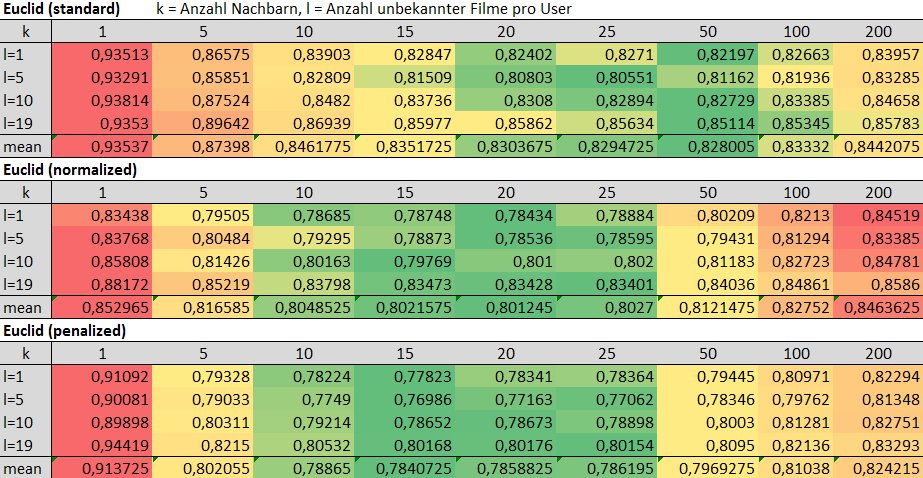
\includegraphics[width=1\linewidth]{ErrorEuclid}
	\caption{MAE im Euklid Algorithmus in Abhängigkeit der Parameter}
	\label{fig:ErrorEuclid}
	
\end{figure}
Die Werte sind mit einer Farbskala von Rot über Gelb nach Grün je Zeile formatiert, um den maximalen Fehler (rot) und den minimalen Fehler (grün) in einem Szenario besser erkennen zu können.\\\\
Wie man an den Tabellen sehen kann, verbessert die Normalisierung den Standard-Euklid-Algorithmus aus \autoref{euclid} . Eine stärkere Verbesserung wird jedoch durch die eingebaute Strafe erzielt. Mit den Parametern $k = 15$ und der Strafe kann der Fehler minimiert werden. In den folgenden Vergleichen werden immer diese Parameter benutzt.
\clearpage

\subsubsection{Wahl von $k$ bei den kNN im Pearson Algorithmus}\label{s.kpearson}
\begin{figure}[h!]
\centering
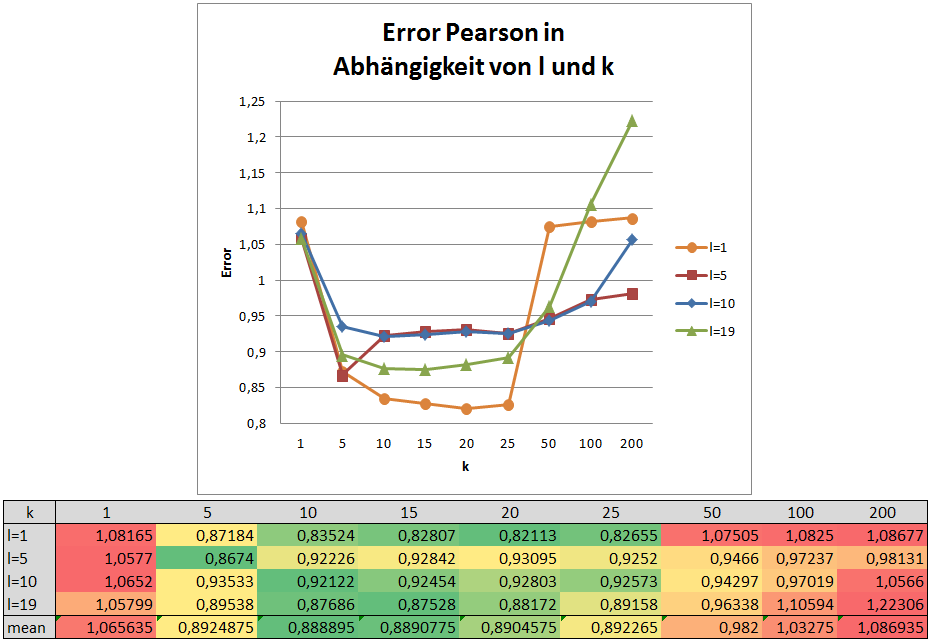
\includegraphics[width=1\linewidth]{ErrorPearsonk}
\caption{MAE im Pearson Algorithmus in Abhängigkeit der Parameter }
\label{fig:ErrorPearsonk}
\end{figure}
Eine Wahl von $k = 10$ nächsten Nachbarn optimiert den Pearson Algorithmus. Im Szenario $l = 1$ zeigt der Algorithmus seine Stärken. Wenn viele Informationen vorhanden sind, können mit dem Pearson Algorithmus gute Bewertungen vorhergesagt werden. Wenn man die mittleren Szenarien $l = 5$ und $l = 10$ mit $l = 19$ vergleicht, fällt auf, dass das letzte Szenario am besten abschneidet. Da hier 19 Fehler berechnet und gemittelt werden. Im Fall $l = 5$ werden nur fünf Fälle verglichen, dadurch entsteht im Mittel eine größere Abweichung zwischen der Vorhersage und der tatsächlich abgegeben Bewertung.
\clearpage

\subsubsection{Wahl von $k$ bei den kNN im Floyd Warshall Algorithmus}\label{s.kflowar}
\begin{figure}[h!]
\centering
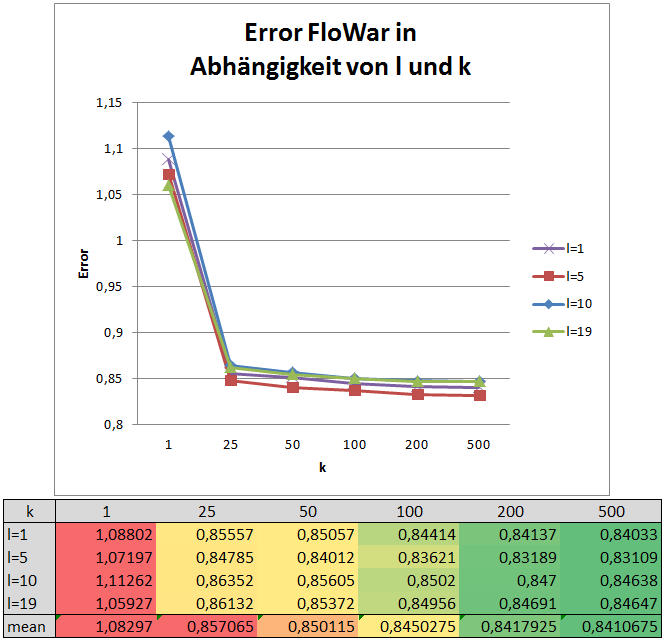
\includegraphics[width=1\linewidth]{ErrorFloWark}
\caption{MAE im Floyd Warshall Algorithmus in Abhängigkeit der Parameter}
\label{fig:ErrorFloWark}
\end{figure}
Man sieht in \autoref{fig:ErrorFloWark}, dass Floyd-Warshall bei großem $k$ (=500) am besten funktioniert. Es wird das Minimum aus den $k$ nächsten Nachbarn und den $n$ nächsten Nachbarn, die den aktuell zu bewertenden Film überhaupt bewertet haben, genommen, um das zu erwartete Rating zu ermitteln. Dies tendiert gegen den Durchschnittswert aller User, die die fehlenden Items bewertet haben. Somit ist der FW-Algorithmus fast gleichzusetzen mit dem Itemmean.
\clearpage

\subsubsection{Wahl von $a$ beim Hybrid Algorithmus}\label{s.alugu}

\begin{figure}[h!]
\centering
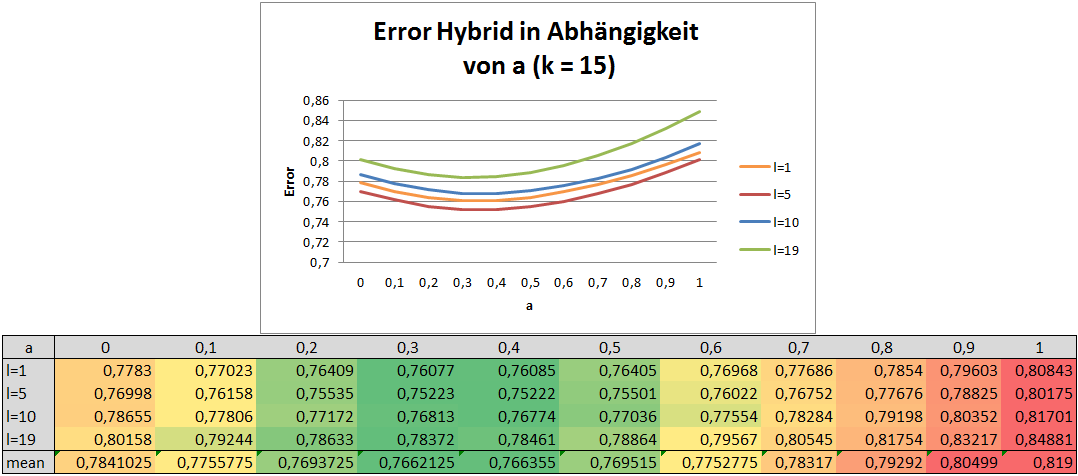
\includegraphics[width=1\linewidth]{ErrorHybrida}
\caption{MAE im Hybrid Algorithmus in Abhängigkeit der Parameter}
\label{fig:ErrorLUSGUSa}
\end{figure}
\FloatBarrier
Ein Verhältnis aus 70\% Euklid und 30\% Slope One minimiert den Fehler. Während der Euklid Algorithmus nur ähnliche Nachbarn untersucht, hilft das Wissen aus dem Item-basierten Algorithmus Slope One den MAE weiter zu minimieren.


\subsection{Auswertung der Fehlerberechnung}\label{s.auswertung}
Neben den sechs genannten Algorithmen (s. \nameref{tab:Liste der Algorithmen}) habe ich noch drei weitere Algorithmen für den Vergleichstest implementiert. Der einfachste, Random, erzeugt einen randomisierten Float zwischen $[1,5]\subset \mathbb{R}$. Usermean $\bar{R}^{user}_{u}$ ermittelt den Durchschnitt des Users, der gerade betrachtet wird. Itemmean $\bar{R}^{item}_{i}$ berechnet die durchschnittliche Bewertung aller User des Items, das gerade im Fokus ist (s. \autoref{definition}). 
Gegen diese drei simplen Algorithmen werden die MAE der sechs oben beschriebenen Funktionen gemessen. Wobei wieder alle vier Szenarien bezüglich des Parameters $l$ betrachtet werden.\\

\begin{figure}[h!]
\centering
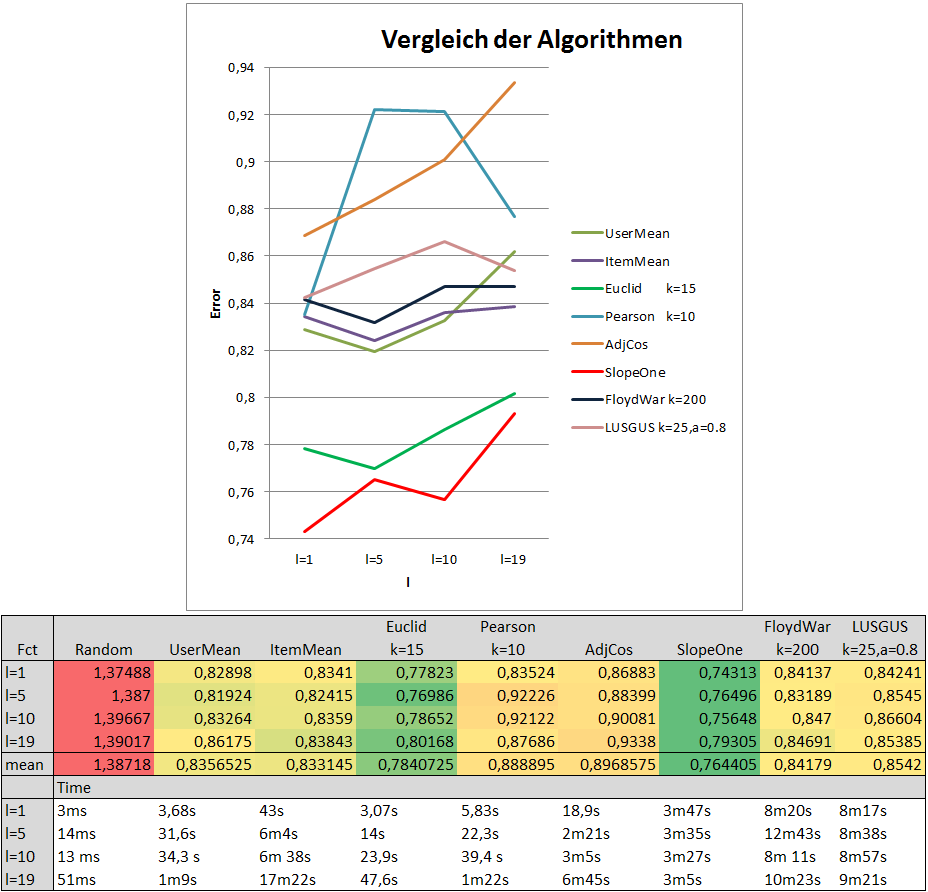
\includegraphics[width=1\linewidth]{Vergleich}
\caption{MAE Vergleich aller Algorithmen}
\label{fig:Vergleich}
\end{figure}
\FloatBarrier
Die Laufzeiten dienen als zusätzlicher Vergleich zwischen den Algorithmen. Die Daten sind in einer Hashmap gespeichert und es wird nur ein Kern der CPU ausgelastet. Durch andere Implementierungen und andere PC-Setups können die Zeiten variieren.\\
Usermean und Itemmean erzielen im Vergleich kein schlechtes Ergebnis, zählen sogar laut MAE mit zu den besten Algorithmen. Usermean ist für Vorhersagen nicht brauchbar, da jedes unbekannte Item das gleiche Rating bekommt. Einen Einsatz findet dieser Algorithmus nur, wenn kein anderer User diesen Film bisher bewertet hat. Bei Itemmean können zwar allgemein beliebte Filme vorgeschlagen werden, die Vorlieben des Users werden aber komplett ignoriert. Pearson erkennt sogar Ähnlichkeiten in relativen Abweichungen und kommt somit mit einem geringem $k$ im k-Nearest-Neighbors aus. Das genaue Gegenteil ist bei Floyd-Warshall der Fall. Der sehr groß eingestellte Parameter $k$ führt dazu, dass FW ähnlich wie Itemmean die bekannten Informationen über den User vernachlässigt. Da mit dem Itemmean eine bessere durchschnittliche Abweichung erzielt wird, als über die entdeckten Pfade zu anderen User. Adjusted Cosine Similarity ist in diesem Test nicht sehr erfolgreich. Obwohl es mit dem gleichen Score arbeitet wie der PCC und dort alle bekannten Informationen über die zwei Items verwendet, können keine guten Vorhersagen erzielt werden. Bessere Vorhersagen erzielt man  mit dem Item-basierten Algorithmus Slope One. Die absolute durchschnittliche Differenz zwischen den Items verwendet alle verfügbaren Informationen aus dem Datensatz. Neben den Differenzen zwischen allen Items muss auch noch eine Frequenzmatrix gespeichert werden. Neue Informationen können dadurch ohne großen Rechenaufwand in die Abstandsmatrix eingearbeitet werden. Die Vorberechnungen im Slope One machen allerdings nur ca. 30 Sekunden der gesamten Zeit aus. Damit braucht der Algorithmus auch recht lange, um Vorhersagen für viele Nutzer gleichzeitig zu berechnen. Der Algorithmus mit dem euklidischen Abstand und Strafe schneidet sehr gut ab und hat dazu sehr kurze Berechnungszeiten. Ein noch besseres Ergebnis liefert das Hybrid Verfahren. Das gemittelte Rating zu 70\% aus dem besten User-basierten (Euklid mit Strafe) und zu 30\% aus dem besten Item-basierten Algorithmus (Slope One) minimiert in diesem Test den MAE. Jedoch verlängert Slope One die Laufzeit immens.\\

\begin{figure}[h!]
	\centering
	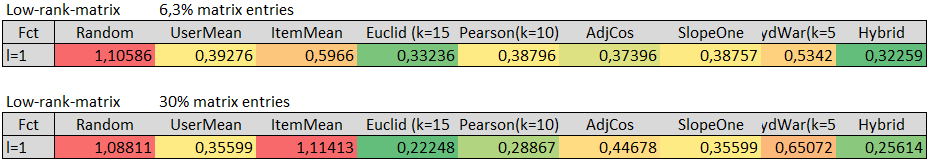
\includegraphics[width=1\linewidth]{bilder/lowrank}
	\caption{MAE Vergleich mit einer Matrix mit niedrigem Rang}
	\label{fig:LowRankMatrix}
\end{figure}
\FloatBarrier
Bei der Konstruktion mit niedrigem Rang erkennt man, dass die User-basierten Algorithmen richtig gut werden. Das ist aber auch zu erwarten, denn die User ähneln sich sehr stark, da sie alle aus einer Kombination aus dreißig Basis-Usern entstanden sind. Die Bewertungen wurden zufällig erstellt, dadurch können auch keine Ähnlichkeiten zwischen den Filmen entstehen. Dies wertet die Item-basierten Algorithmen zusätzlich ab. Sind viele Informationen bekannt, ändert sich nicht viel an der Reihenfolge der Algorithmen.\\
Einen Vergleich zu der realen Datenbank von MovieLens kann man nur mit Vorsicht tätigen. Wenn man die Histogramme der beiden Matrizen betrachtet, wird klar, dass die Konstruktion der Matrix mit niedrigem Rang nicht sehr nah an die Verteilung der MovieLens-Daten heran kommt.
\begin{figure}[h!]
	\centering
	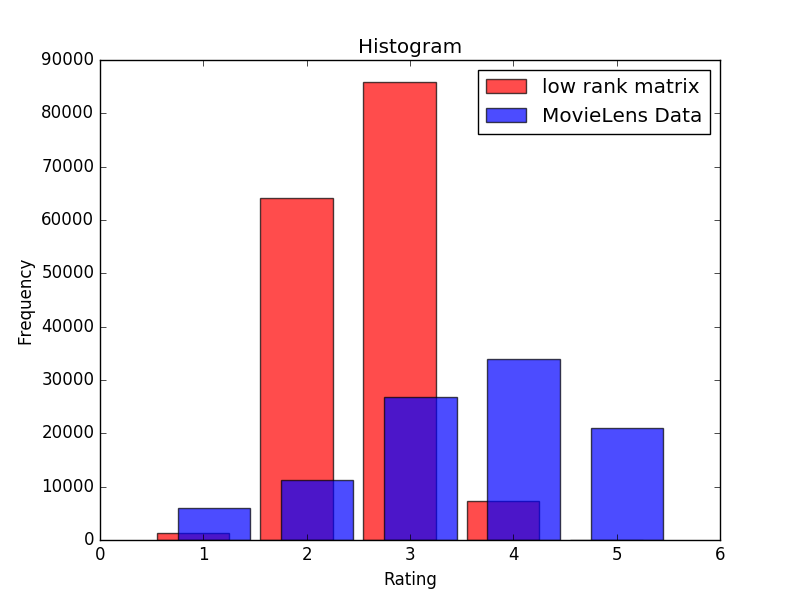
\includegraphics[width=1\linewidth]{histogram}
	\caption{Histogramm Vergleich}
	\label{fig:histogram}
\end{figure}
\FloatBarrier
Beim Versuch die Bewertungen gleichmäßiger zu verteilen, zerstört man die lineare Abhängigkeit der Zeilen. Doch genau diese Eigenschaft der Bewertungen wollte ich mit diesem Test überprüfen. Überraschend ist die Verteilung der MovieLens-Daten. Ich hätte erwartet, dass die 1 häufiger von enttäuschten Usern als negative Bewertung benutzt wird.

\begin{figure}[h!]
	\centering
	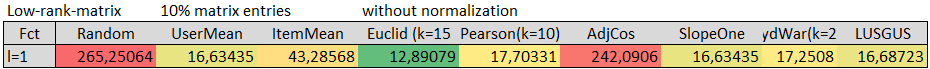
\includegraphics[width=1\linewidth]{lowranknotnorm}
	\caption{MAE Vergleich ohne Normalisierung}
	\label{fig:LowRankMatrixnotnorm}
\end{figure}
\FloatBarrier
In den Daten in \autoref{fig:LowRankMatrixnotnorm} wurde bewusst vermieden, die Bewertungen wieder in den Wertebereich ${1,2,3,4,5}$ zu normieren. Dadurch wird die lineare Abhängigkeit der Zeilen nicht zerstört. Diese erzielten Fehler können deshalb nicht mit den anderen Szenarien verglichen werden. Was man aber erkennen kann, dass die User-basierten Verfahren sehr viel besser abschneiden, als der Item-basierte Algorithmus Adjusted Cosine Similarity. Slope One kann auch hier mit den vollen Informationen der Matrix ein sehr gutes Ergebnis erzielen.
\clearpage
%\section{Quellcode}





%%%%%%%%%%%%%%%%%%%%%%%%%%%%%%%%%%%%%%%%%%%%%%%%%%%%%%%%%%%%%%%%%%%%%%%%
%%%% ENDE TEXTTEIL %%%%%%%%%%%%%%%%%%%%%%%%%%%%%%%%%%%%%%%%%%%%%%%%%%%%%
%%%%%%%%%%%%%%%%%%%%%%%%%%%%%%%%%%%%%%%%%%%%%%%%%%%%%%%%%%%%%%%%%%%%%%%%

\clearpage

% Entfernen Sie das Kommentar aus der nachfolgenden Zeile, falls Sie einen Anhang in der Arbeit verwenden wollen. Beachten Sie, dass Sie sich im Verlauf der Arbeit mit \ref{...} (z.B. \ref{anhang:zusatz1}) auf den Anhang beziehen.
\newpage
\appendix
\section{Anhang: Quellcode}

Da ich vor Beginn dieser Arbeit noch nicht mit Python gearbeitet habe und mit der Syntax noch nicht vertraut war, habe ich mich dazu entschlossen als Start meines Quellcodes, die Recommender Klasse von Ron Zacharski zu nutzen. In seinem Buch "`A Programmer's Guide to Data Mining: The Ancient Art of the Numerati"' \cite{G2DM} stellt er neben den Erklärungen auch Python Quellcode \footnote{\url{https://github.com/zacharski/pg2dm-python}} zur Verfügung. In Chapter 3 befindet sich die Python Datei "recommender3.py". Darin enthalten sind der Import der Movie-Lens-Daten, der Pearson und der Slope One Algorithmus. Des weiteren befindet sich die Funktion computeSimilarity(band1, band2, userRatings) in der Datei "cosineSimilarity.py". Diese Funktion war meine Ausgangslage, um das Verfahren Adjusted Cosine Similarity zu implementieren.\\
Den Code habe ich an meine Bedürfnisse angepasst, damit ich den automatisierten Test mit den Testdaten ausführen konnte. Für diese Zwecke habe ich die Testklasse erstellt. Mit der Funktion $\mathrm{testit}(\mathrm{self}, \mathrm{fct}, k=10, a=0.5)$ kann man den Testlauf für eine der Verfahren starten. Der Parameter $k$ entscheidet die Anzahl der Nachbarn, $a$ wird als Parameter für den Hybrid Modus benötigt. 
\begin{equation}
\begin{aligned}
\mathrm{fct} \in \{\mathrm{'random', 'itemmean', 'usermean', 'euclid', 'pearson',}\\ \mathrm{'slopeone', 'floydwarshall', 'lusgus', 'adjcos'}\}
\end{aligned}
\end{equation}
Der Quellcode und der MovieLens-Datensatz ist online in meinem Github Repository \footnote{\url{https://github.com/kralle71/Collaborative-Filtering}} zu finden.


\subsection{Übersicht aller Funktionen} \label{anhang:übersicht}
\lstset{%
	breaklines=true
}
\lstinputlisting[language=Python]{CollaborativeFiltering-Summary.py}

\clearpage

\subsection{Quellcode} \label{anhang:quellcode}

\lstinputlisting[language=Python]{CollaborativeFiltering.py}


\clearpage

\bibliography{references}
\bibliographystyle{alphadin}
%\vspace*{\fill}

\clearpage

\listoffigures

\listoftables



%\pagebreak

%\printindex
\end{document}
